正文表格对每个测试设置先计算八项指标，再在同类设置内等权平均。ID与复杂度各包含三组来源划分，整域OOD包含三组留出学科，极限OOD包含两个迁移方向。完整单组结果见附录。所有99组模型评价均通过原始字节与字符串精确保真检查。
\subsection{全领域新来源：压缩、命令与结构的取舍}
\par\begin{table}[H]\centering\small
\caption{全领域新来源测试：三个来源划分的均值。百分比列的单位均为\%。}\label{tab:id}
\begin{tabular}{lrrrrrrrr}\toprule
模型 & T/B $\dn$ & Cmd $\up$ & Num $\up$ & Cross $\dn$ & AST-A $\up$ & Used & $\eta_{2.5}$ $\up$ & 速度 $\up$ \\\midrule
Hard AST-BPE & 0.4181 & 92.28 & 96.87 & \textbf{7.71} & \textbf{74.71} & 74.74 & 62.88 & 14.81 \\
AST-v4 & 0.4006 & 99.01 & 96.87 & 8.09 & 73.33 & 76.76 & 62.53 & \textbf{32.42} \\
Boundary AST & \textbf{0.3799} & \textbf{99.73} & 96.37 & 17.50 & 39.28 & 67.97 & 69.69 & 29.36 \\
Math-atom BPE & 0.3830 & \textbf{99.73} & 96.37 & 18.18 & 38.23 & 68.03 & 70.36 & 10.00 \\
Byte BPE & 0.4105 & 36.27 & 96.37 & 25.17 & 24.23 & 78.26 & \textbf{75.16} & 8.49 \\
SP Unigram & 0.4783 & 4.18 & 97.42 & 19.80 & 28.55 & 71.65 & 59.96 & 23.76 \\
\midrule
Qwen2.5 & 0.5261 & 2.02 & 96.37 & 19.98 & 31.51 & 1.02 & 32.99 & 3.15 \\
Llama 3 & 0.5228 & 2.02 & \textbf{99.23} & 20.14 & 29.06 & 1.30 & 33.52 & 9.00 \\
o200k & 0.5174 & 2.62 & \textbf{99.23} & 20.58 & 27.74 & 0.81 & 32.63 & 14.28 \\
\bottomrule\end{tabular}
\end{table}\par

Boundary AST的T/B为0.3799，相对Byte BPE减少7.45\%，相对硬AST-BPE减少9.12\%。Math-atom BPE为0.3830；两者共享词表后，软结构路径使T/B进一步减少0.80\%。Boundary AST与Math-atom BPE的Cmd均值分别为99.73\%与99.73\%，表明数学原子初始化直接改善了完整命令的表示。
硬约束的优势体现在结构列：Hard AST-BPE与AST-v4的AST-A分别为74.71\%和73.33\%，Cross分别为7.71\%和8.09\%；Boundary AST的对应值为39.28\%和17.50\%。因此压缩最优路径与最多复合节点边界是不同目标，硬／软约束提供不同工作点。
硬约束使用原生算术／绑定语法前端，Cross与AST-A使用独立KaTeX参考；两个前端生成的语法跨度有差异，表中的Cross测量所有模型与同一外部参考的一致性。
Llama 3与o200k的Num均值为99.23\%与99.23\%，Byte BPE的Rényi效率为75.16\%，这些列保留了通用数字分组和字节BPE分布性质的优势。
\begin{figure}[htbp]\centering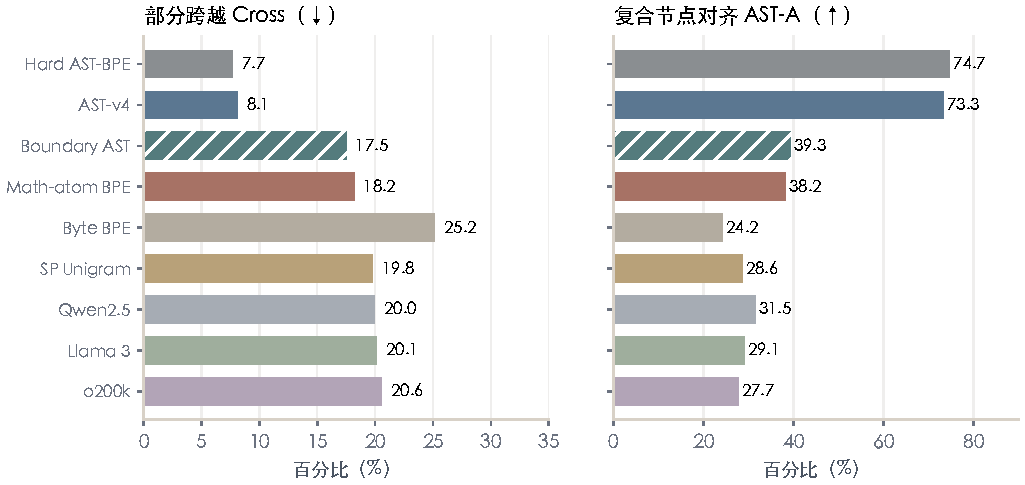
\includegraphics[width=\linewidth]{figures/structure.pdf}\caption{全领域测试中的两种结构测量。柱形为三个来源划分的均值，数值单位为\%。}\label{fig:structure}\end{figure}
\subsection{整域与极限OOD：词表的跨学科迁移}
\par\begin{table}[H]\centering\small
\caption{三个整域留出设置的等权均值。}\label{tab:ood}
\begin{tabular}{lrrrrrrrr}\toprule
模型 & T/B $\dn$ & Cmd $\up$ & Num $\up$ & Cross $\dn$ & AST-A $\up$ & Used & $\eta_{2.5}$ $\up$ & 速度 $\up$ \\\midrule
Hard AST-BPE & 0.4287 & 91.60 & 97.54 & \textbf{7.32} & \textbf{76.29} & 75.88 & 61.52 & 14.67 \\
AST-v4 & 0.4089 & 98.90 & 97.60 & 7.81 & 74.69 & 78.16 & 61.34 & \textbf{30.67} \\
Boundary AST & \textbf{0.3869} & \textbf{99.70} & 97.08 & 17.26 & 40.08 & 71.39 & 69.31 & 27.80 \\
Math-atom BPE & 0.3908 & \textbf{99.70} & 97.08 & 17.79 & 38.81 & 71.48 & 69.65 & 9.39 \\
Byte BPE & 0.4161 & 46.20 & 97.08 & 23.47 & 26.13 & 79.49 & \textbf{74.39} & 7.73 \\
SP Unigram & 0.4890 & 3.09 & 97.92 & 19.49 & 28.77 & 72.56 & 59.76 & 22.57 \\
\midrule
Qwen2.5 & 0.5238 & 2.10 & 97.08 & 19.54 & 32.22 & 1.38 & 33.07 & 3.17 \\
Llama 3 & 0.5211 & 2.10 & \textbf{99.36} & 19.66 & 30.09 & 1.90 & 33.59 & 8.80 \\
o200k & 0.5169 & 2.52 & \textbf{99.36} & 20.04 & 28.99 & 1.19 & 32.81 & 14.01 \\
\bottomrule\end{tabular}
\end{table}\par

\par\begin{table}[H]\centering\small
\caption{分析／方程与代数／数论双向极限OOD的均值。}\label{tab:extreme}
\begin{tabular}{lrrrrrrrr}\toprule
模型 & T/B $\dn$ & Cmd $\up$ & Num $\up$ & Cross $\dn$ & AST-A $\up$ & Used & $\eta_{2.5}$ $\up$ & 速度 $\up$ \\\midrule
Hard AST-BPE & 0.4374 & 87.14 & 96.10 & \textbf{7.30} & \textbf{78.48} & 75.44 & 60.84 & 15.10 \\
AST-v4 & 0.4220 & 98.27 & 96.10 & 7.61 & 77.80 & 76.07 & 59.94 & \textbf{30.72} \\
Boundary AST & \textbf{0.3919} & \textbf{98.58} & 95.29 & 16.59 & 42.90 & 74.61 & 69.38 & 27.98 \\
Math-atom BPE & 0.3967 & \textbf{98.58} & 95.29 & 16.94 & 41.79 & 74.46 & 69.83 & 9.56 \\
Byte BPE & 0.4286 & 45.84 & 95.34 & 21.52 & 31.40 & 77.05 & \textbf{72.69} & 7.71 \\
SP Unigram & 0.5019 & 3.38 & 96.39 & 18.80 & 30.75 & 71.34 & 61.26 & 22.21 \\
\midrule
Qwen2.5 & 0.5265 & 1.95 & 95.28 & 19.22 & 34.52 & 1.40 & 33.21 & 3.13 \\
Llama 3 & 0.5219 & 1.95 & \textbf{99.01} & 19.40 & 30.67 & 1.98 & 33.78 & 8.76 \\
o200k & 0.5183 & 2.54 & \textbf{99.01} & 19.71 & 29.61 & 1.25 & 33.04 & 14.30 \\
\bottomrule\end{tabular}
\end{table}\par

整域 OOD中，T/B最小者为Boundary AST（0.3869）。Boundary AST的Cmd为99.70\%，AST-v4的AST-A为74.69\%。完整留出领域和方向分别列于表\ref{tab:splits}与附录。
极限 OOD中，T/B最小者为Boundary AST（0.3919）。Boundary AST的Cmd为98.58\%，AST-v4的AST-A为77.80\%。完整留出领域和方向分别列于表\ref{tab:splits}与附录。
\subsection{简单到复杂：长度与层次变化}
\par\begin{table}[H]\centering\small
\caption{简单公式训练、复杂公式测试：三个来源划分均值。}\label{tab:complexity}
\begin{tabular}{lrrrrrrrr}\toprule
模型 & T/B $\dn$ & Cmd $\up$ & Num $\up$ & Cross $\dn$ & AST-A $\up$ & Used & $\eta_{2.5}$ $\up$ & 速度 $\up$ \\\midrule
Hard AST-BPE & 0.4226 & 86.17 & 96.91 & \textbf{7.63} & \textbf{74.66} & 73.11 & 61.78 & 16.38 \\
AST-v4 & 0.4022 & 98.81 & 96.93 & 8.06 & 73.25 & 74.25 & 61.87 & \textbf{41.04} \\
Boundary AST & \textbf{0.3802} & \textbf{99.62} & 96.13 & 17.96 & 38.18 & 67.25 & 69.29 & 36.33 \\
Math-atom BPE & 0.3852 & \textbf{99.62} & 96.13 & 19.16 & 36.13 & 67.06 & 69.41 & 11.88 \\
Byte BPE & 0.4084 & 64.80 & 96.13 & 21.50 & 29.17 & 76.89 & \textbf{72.04} & 9.56 \\
SP Unigram & 0.5020 & 2.72 & 97.42 & 16.00 & 37.73 & 67.84 & 53.34 & 29.80 \\
\midrule
Qwen2.5 & 0.5142 & 2.73 & 96.13 & 20.40 & 30.86 & 0.87 & 32.83 & 3.47 \\
Llama 3 & 0.5110 & 2.73 & \textbf{99.14} & 20.58 & 28.38 & 1.09 & 33.37 & 10.12 \\
o200k & 0.5058 & 3.29 & \textbf{99.14} & 21.09 & 26.98 & 0.68 & 32.49 & 16.31 \\
\bottomrule\end{tabular}
\end{table}\par

只在简单公式上构建词表后，Boundary AST在复杂公式上的T/B为0.3802，相对Byte BPE减少6.91\%，Cmd为99.62\%。AST-v4的AST-A为73.25\%，编码速度为41.04 MiB/s。该设置同时改变未见来源与公式句法复杂度。
\begin{figure}[htbp]\centering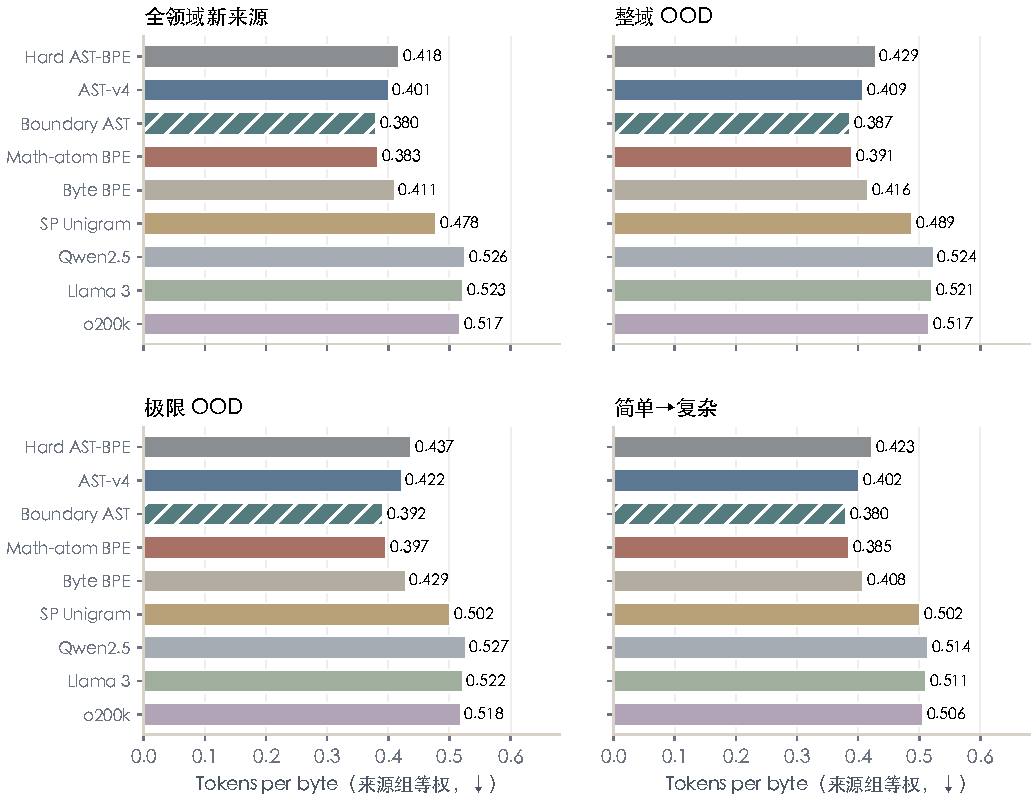
\includegraphics[width=\linewidth]{figures/compression.pdf}\caption{四类泛化测试的压缩结果。各柱为同类设置等权均值；横轴从零开始，越短表示每字节所需token越少。}\label{fig:compression}\end{figure}
\subsection{运行速度与词表使用}
全领域测试中，AST-v4、Boundary AST、Math-atom BPE和Byte BPE的平均完整编码速度分别为32.42、29.36、10.00与8.49 MiB/s。AST-v4和Boundary AST在C前端中融合解析、trie与路径搜索；速度比较涵盖全部这些步骤。Used以完整ID空间为分母，通用词表与数学专用词表在本公式集上的实际使用比例直接列于各表。
\begin{figure}[htbp]\centering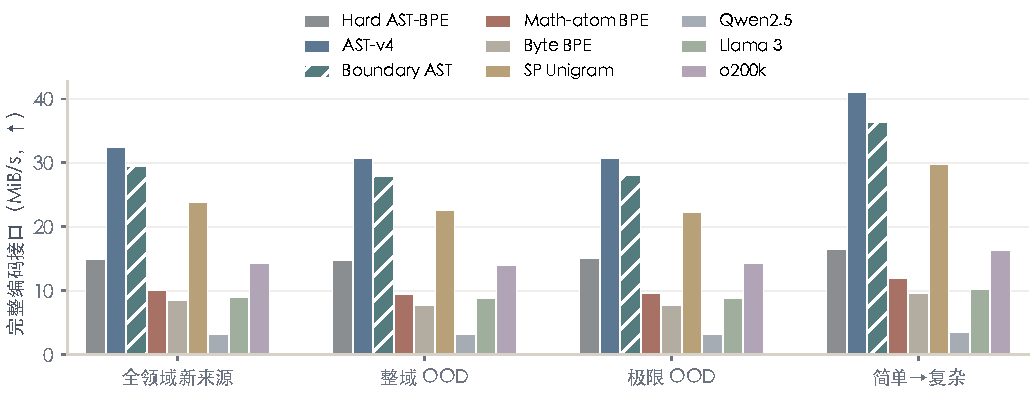
\includegraphics[width=\linewidth]{figures/speed.pdf}\caption{相同测试输入、逐公式完整接口和七轮交错计时下的编码速度。每类对其设置等权平均。}\label{fig:speed}\end{figure}
\subsection{分指标排序与模型选择}
Boundary AST在11个单独设置中均取得最低T/B。以四类测试分别等权后得到分指标前三名，见表\ref{tab:ranks}；数值相同时并列，表格展示顺序沿用模型列表。Used描述测试集使用词表的比例。压缩、命令和数字完整性、语法对齐、分布均匀性与速度分别报告。
\par\begin{table}[H]\centering\small\caption{四类测试等权后的分指标排序，等值并列。Used不用于质量排序。}\label{tab:ranks}\begin{tabularx}{\linewidth}{lYYY}\toprule 指标&第一梯队&第二梯队&第三梯队\\\midrule
T/B & Boundary AST 0.3847 & Math-atom BPE 0.3889 & AST-v4 0.4084 \\
Cmd & Boundary AST／Math-atom BPE 99.41\% & AST-v4 98.75\% & Hard AST-BPE 89.30\% \\
Num & Llama 3／o200k 99.19\% & SP Unigram 97.28\% & AST-v4 96.87\% \\
Cross & Hard AST-BPE 7.49\% & AST-v4 7.89\% & Boundary AST 17.33\% \\
AST-A & Hard AST-BPE 76.04\% & AST-v4 74.77\% & Boundary AST 40.11\% \\
$\eta_{2.5}$ & Byte BPE 73.57\% & Math-atom BPE 69.81\% & Boundary AST 69.42\% \\
速度 & AST-v4 33.71 & Boundary AST 30.37 & SP Unigram 24.59 \\
\bottomrule\end{tabularx}\end{table}\par
下游实验保留软约束Boundary AST与硬约束AST-v4两个结构工作点，以Math-atom BPE分离词表与分割贡献，并保留Byte BPE、SP Unigram及三个通用词表作为参照。标准硬AST-BPE给出不预留数学原子的硬结构基线。
